\qns{RLC circuit}

Consider the circuit shown below:

\begin{center}
    \begin{circuitikz}[scale=0.8]
        \draw (-1,4)
        to [V = $V_s$,i=$i_s$] (-1,0)
        (-1,4) to [switch, l^=\mbox{$t = 0$} ] (1,4)
        to [opening switch,l^=\mbox{$t = 0$} ] (1,0)
        (1,4) to [R = $R_s$] (4,4)
        to [C = $C$,i=$i_C$] (4,0)
        to [short] (-1,0)
        (4,4) to [short] (8,4)
        to [L = $L$,i=$i_L$, v = $V_{out}$] (8,0)
        to [short] (-1,0);
    \end{circuitikz}
\end{center}

Assume the circuit reaches steady state for $t<0.$ At time $t = 0,$ the switch changes state and connects to the voltage source $V_s$.

\meta {
    Explain what it means when the circuit reaches steady state.
}

\begin{enumerate}

	\qitem \textbf{Find the differential equation for $V_{out}$ for $t\geq0$.} \textit{Hint: Write out the KCL equation.}

    \ws {
        \vspace{75px}
    }

	\meta {
		It might not be intuitive at first to take the derivative, however, we want to find $V_{out} = V_L$ and remember that the voltage-current relationship of an inductor is $V_L = L \ddt{i_L(t)}{t}.$
		Our KCL equation is in terms of $i_L(t)$ we'll take a derivative to substitute the relation above.
	}

	\sol{
	We first see that
	$$i_s = i_R = i_C + i_L$$
	We will take the derivative to get:
	$$\ddt{i_s}{t} = \ddt{i_C}{t} + \ddt{i_L}{t}$$
	From the voltage-current relations, we know that:
	$$i_s = \frac{V_s-V_{out}}{R_s}, i_C = C \ddt{V_{out}}{t}, \ddt{i_L(t)}{t} = \frac{V_{out}}{L}$$
	Taking derivatives and substituting we get:
	$$\frac{d^2V_{out}}{dt^2}+\frac{1}{R_sC}\frac{dV_{out}}{dt}+\frac{1}{LC}V_{out} = 0$$
% \[i_s=i_c+i_l\]
% Using $i_c=C\frac{dV_{out}}{dt}$ and Ohm's law:
% \[\frac{V_s-V_{out}}{R_s}=C\frac{dV_{out}}{dt}+i_l\]

% Substituting $V_{out}=L\frac{di_l}{dt}$
% \[\frac{V_s}{R_s}=\frac{L}{R_s}\frac{di}{dt}+LC\frac{d^2i}{dt^2}+i_l\]
% \[\frac{V_s}{R_sLC}=\frac{1}{R_sC}\frac{di}{dt}+\frac{d^2i}{dt^2}+\frac{i_l}{LC}\]
% Since we have $V_{out}=L\frac{di_l}{dt}$, we take the derivative of both sides to get an equation in the form of $V_{out}$
% \[0=\frac{1}{R_sC}\frac{d^2i}{dt^2}+\frac{d^3i}{dt^3}+\frac{1}{LC}\frac{di_l}{dt}\]
% \[0=\frac{d^2V_{out}}{dt^2}+\frac{1}{R_sC}\frac{dV_{out}}{dt}+\frac{1}{LC}V_{out}\]
    }
    \qitem We will define our state variable $\vec{x}(t) = \begin{bmatrix} V_{out}(t) \\ \frac{d}{dt} V_{out}(t) \end{bmatrix}$.

    \textbf{Set up a system of differential equations in the form $\vec{x}(t) = A \vec{x}(t)$. What are its initial conditions $\vec{x}(0)$?}

    \ws{
        \vspace{75px}
    }
    \sol{
    We know that at $t=0,$ $V_{out}=0$, $i_C=0$, and $i_L=0$. We also know that the voltage on a capacitor and the current through an inductor can't change instantaneously, so it follows that
    $$\vec{x}(0) = \begin{bmatrix} V_{out}(0)=0 \\ \ddt{V_{out}(t)}{t}(0)=0 \end{bmatrix}.$$
    Putting the differential equation in state-space we see that:
    $$\ddt{}{t} \vec{x}(t) =
    \begin{bmatrix} \ddt{V_{out}(t)}{t} \\ \frac{d^2V_{out}}{dt^2} \end{bmatrix} =
    \begin{bmatrix} \ddt{V_{out}(t)}{t} \\ -\frac{1}{R_sC} \frac{dV_{out}}{dt} - \frac{1}{LC} V_{out} \end{bmatrix} =
    \begin{bmatrix} 0 & 1 \\ -\frac{1}{LC} & -\frac{1}{R_sC} \end{bmatrix}\begin{bmatrix} V_{out}(t) \\ \ddt{V_{out}(t)}{t} \end{bmatrix} =\begin{bmatrix} 0 & 1 \\ -\frac{1}{LC} & -\frac{1}{R_sC} \end{bmatrix} \vec{x}$$
    }

	\qitem \textbf{Find the eigenvalues of $A$.}

    \ws {
        \vspace{75px}
    }

    \sol {
    To find the eigenvalues, we take a look at the determinant of $A - \lambda I.$
    $$\text{det}\mathbf
    {\begin{bmatrix}
        -\lambda & 1 \\
        -\frac{1}{LC} & -\frac{1}{R_s C} - \lambda \end{bmatrix}}
    = (- \lambda)(-\frac{1}{R_s C} - \lambda) + \frac{1}{LC} = \lambda^2 + \frac{1}{R_s C} \lambda + \frac{1}{LC}$$
    Therefore using the quadratic formula,
    $$\lambda = -\frac{1}{2 R_s C} \pm \frac{1}{2} \sqrt{(\frac{1}{R_s C})^2 - \frac{4}{LC}}$$
    }

    \qitem \textbf{When are the eigenvalues real, complex, and distinct?} \textit{Hint: When is there a negative under the square root?}

    \ws {
        \vspace{100px}
    }

    \sol {
        The main term that will determine whether the eigenvalues are real or complex is the $\sqrt{(\frac{1}{R_s C})^2 - \frac{4}{LC}}$ term.
        \begin{enumerate}
        \item If this term is greater than 0, or if $R_s < \sqrt{\frac{L}{4C}},$ then the eigenvalues must be real and distinct.
        \item If this term less than 0, or if $R_s > \sqrt{\frac{L}{4C}},$ then the eigenvalues must be complex.
        \item If this term is equal to 0, or if $R_s = \sqrt{\frac{L}{4C}},$ then there will be a unique real eigenvalue.
        \end{enumerate}
    }


    \qitem
    Based on the eigenvalues, we can describe the shape of the graph of $V_{out}$ from the RLC circuit.
    \begin{itemize}
    \item \textbf{Case I:} If the eigenvalues are real and distinct, the solution will look like a decaying exponential.
    \item \textbf{Case II:} If the eigenvalues are complex, the solution will have a decaying exponential envelope with oscillations inside.
    \item \textbf{Case III:} If there is a unique real eigenvalue, the solution will look like a decaying exponential with rate of decay faster than that of (i).
    \end{itemize}
    Draw examples of what case I, II, and III look like.
    Can you explain the intuition behind why these graphs look the way they do?
    \textit{Hint: Euler's Formula states that $e^{i\theta} = \cos{\theta} + i\sin{\theta}$}

    % https://tex.stackexchange.com/questions/454298/damped-oscillation-graph-in-latex
    \sol{
    The graph below illustrates what a potential example may look like where red is a decaying exponential.
    Blue represents a situation where we have a decaying exponential with oscillations.
    Black represents a decay with a faster rate of decay than red.

    For intuition on the oscillations, the reasoning lies behind Euler's theorem.
    Specifically, Euler's states that $e^{i\theta} = \cos\theta + i\sin\theta$.
    This means that if the magnitude of the exponential is decaying over time, but the eigenvalue is complex, we'll have a decaying sum of sines and cosines.
    In fact, if our exponential weren't decaying, we'd have everlasting oscillations!
    This idea is explored more in the homework.

    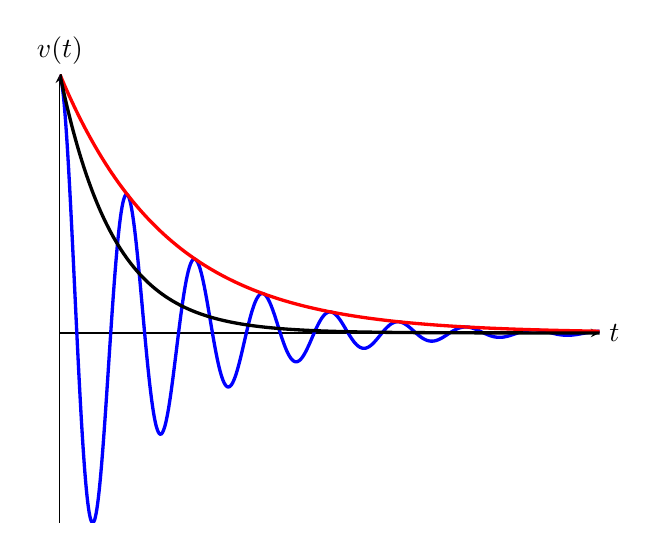
\begin{tikzpicture}
        \begin{axis}[domain=0:5,samples=501,axis lines=center,
        xtick=\empty,ytick=\empty,
        xlabel={$t$},xlabel style={anchor=west},
        ylabel={$v(t)$},ylabel style={anchor=south}]
        \addplot[color=blue,no marks,very thick,smooth] {(exp(-x)*cos(10*deg(x)))};
        \addplot[color=red,no marks, very thick, smooth] {(exp(-x))};
        \addplot[color=black, no marks, very thick, smooth] {(exp(-2 * x))};
        \end{axis}
    \end{tikzpicture}
    }

    \meta {
        Draw out these plots for your students for the three cases.
    }

    \end{enumerate}


%     Solve the differential equation. Considering all of these cases.

% 	\sol{The general solution to the trsolient equation of this form is \[V_{out}(t)=K_1e^{\lambda_1 t}+K_2e^{\lambda_2 t}\]
% 	where
% 	\[\lambda_1=-\alpha +\sqrt{\alpha^2-\omega_0^2}  \]
% 	\[\lambda_2=-\alpha -\sqrt{\alpha^2-\omega_0^2}\]
% 	In this case,
% 	\[\alpha=\frac{1}{2R_sC}\]
% 	\[\omega_0=\frac{1}{\sqrt{LC}}\]
% 	Now to find the constants $K_1$ and $K_2$, we use the initial conditions for $v_{out}(0)$ and $\frac{dv_{out}(0)}{dt}$ and set the general solution to these values:
% 	\begin{align*}
% 		\frac{dv_{out}(0)}{dt}=\frac{V_s}{R_sC}&=K_1\lambda_1+K_2\lambda_2 \\
% 	v_{out}(0)=0&=K_1+K_2 \\
% 	\frac{V_s}{R_sC}&=-K_2\lambda_1+K_2\lambda_2 \\
% 	K_2&=\frac{V_s}{R_sC(\lambda_2-\lambda_1)} \\
% 	K_1&=-\frac{V_s}{R_sC(\lambda_2-\lambda_1)}
% 	\end{align*}
% 	Finally, plugging back into the general solution:
% 	\[V_{out}(t)=-\frac{V_s}{R_sC(\lambda_2-\lambda_1)}e^{\lambda_1 t}+\frac{V_s}{R_sC(\lambda_2-\lambda_1)}e^{\lambda_2 t}\]

% 	For the $\lambda_1=\lambda_2$, which happens in a critically damped system, the general solution is:
% \[V_c=K_1e^{\lambda t}+tK_2e^{\lambda t}\]
% and
% \[\frac{dV_c}{dt}=K_1\lambda e^{\lambda t}+K_2e^{\lambda_t}+t K_2 \lambda e^{\lambda t}\]
% so when plugging our initial conditions into these equations
% \begin{align*}
% V_{out}(0)&=0=K_1 \\
% \frac{dV_c (0)}{dt}&=\frac{V_s}{R_sC}=K_1\lambda+K_2 \\
% K_2&= \frac{V_s}{R_sC} \\
% K_1&=0 \\
% K_2&=\frac{V_s}{R_sC}
% \end{align*}
